\documentclass[a4paper,man,natbib,floatsintext,12pt]{apa7}

\usepackage[english]{babel} %character and hyphenation rules specific to the language you choose
%\usepackage[utf8x]{inputenc}
\usepackage{graphicx}
\usepackage{color}
\usepackage{tikz}
\usepackage{float}
\usepackage{amsmath}
\usepackage{blindtext}
\usepackage{tabularx} %great for APA-style Tables
\usepackage{siunitx} % Required for good table alignmen
\sisetup{
  round-mode          = places, % Rounds numbers
  round-precision     = 2, % to 2 places
}
\usepackage{multirow}
\usepackage{booktabs}
\usepackage{wrapfig}
\usetikzlibrary{shapes,decorations,arrows,calc,arrows.meta,fit,positioning}
\tikzset{
    -Latex,auto,node distance =1 cm and 1 cm,semithick,
    latent/.style ={ellipse, draw, minimum width = 0.7 cm},
    observed/.style ={rectangle, draw},
    bidirected/.style={Latex-Latex,dashed},
    el/.style = {inner sep=2pt, align=left, sloped}
}
\newcommand{\sigFtest}[4]{\textit{F}(#1,#2) = #3, \textit{p}$<$#4}
\newcommand{\nonsigFtest}[3]{\textit{F}(#1,#2) = #3, \textit{p}$>$.05}


\title{Neural Resonance Profiling: Oscillatory Preferences as Biomarkers for Mild Cognitive Impairment }
\shorttitle{Neural Resonance Profiling: MCI}
\author{Kathryn A. Gour}
\affiliation{College of William \& Mary}
\journal{The Best Psychology Journal EVER!}
\abstract{\blindtext}
\keywords{APA style, demonstration}
\authornote{I would like to thank the CPL and my puppy, Austin.}
\leftheader{Alternate page header in man mode}

%-------------- END PREAMBLE  -------------------


\begin{document}

\maketitle  %Insert my APA style title page

\section{Introduction}
\par Auditory stimuli across frequency bands should establish a rhythm for oscillatory signals to entrain, providing opportunities to measure neural resonance. This phenomenon of neural resonance means that neural networks are in a steady state of excitability when stimuli are presented, and certain stimulation frequencies should induce ‘resonance peaks’ \citep{calderone2014entrainment}. Understanding how individual differences in neural resonance entrainment are related to ASD is critical because research suggests that neural resonance can be affected by factors like dendritic branching and network complexity, which can increase with age and cause a decrease in oscillatory coherence and synchronization, affecting ASD populations disproportionately \citep{laudanski2014spatially, martorell2019multi}. Exploring oscillatory power, neural resonance, and individual variability in neurodivergent and neurotypical individuals is critical for understanding how ASD affects social, affective, and cognitive functions. 
\par In the current study, binaural beats were used to induce neural entrainment within the frequency range of 1 to 50 Hz. If binaural beats are ineffective at inducing entrainment, one would expect no differences in oscillatory power at the binaural beat frequency between EEG recorded during the binaural beat stimulation and a pure tone condition (beat frequency = 0). Likewise, oscillatory power, reflecting neural resonance, would be expected to increase during binaural beat stimulation in participants with higher levels of ASD traits such as aloofness, comparable to those with lower levels of these traits, suggesting no significant difference in neural resonance profiles based on ASD trait severity. The first alternative hypothesis is that binaural beat stimulation does induce a significant increase in oscillatory power compared to the pure tone. This hypothesis means that there would be peak frequencies for different binaural beat stimulation frequencies (1-50 Hz) that are significantly higher in amplitude compared to pure tone stimulation frequencies (100 Hz). The second alternative hypothesis is that there are significant differences between the resonance profiles of participants high on the ASD scale versus low on the ASD scale. This hypothesis means that we would expect significantly higher peak frequencies in different canonical frequency bands (i.e., Alpha, Beta, Theta, Gamma, and Delta) for participants scoring higher on the ASD scale. 


\section{Method}
\subsection{Participants}
\par Younger adults (N = 57) were recruited from William \& Mary’s SONA (i.e., research participation) system. The sample was 72\% female, and the average age was 18.8 years (SD = .94). Participants were offered class credit for the approximately 75-minute-long procedure. Participants were excluded if they self-reported any auditory impairments, a history of stroke, or neuropsychiatric or neurodegenerative disorder. Five participant data files were also excluded from the analysis because of excessive noise in the EEG recordings (i.e., movement affected brain data). The experiment was conducted with the informed consent of each participant following a College of William \& Mary-approved IRB protocol (PHSC-2024-08-28-17197). 
\subsection{Procedure \& Stimuli }
Binaural beats were used to drive neural entrainment at frequencies between 1 Hz and 50 Hz, increasing in 1 Hz increments, centered around a frequency of 440 Hz. All auditory stimuli were generated using MATLAB (v2024a) and presented with ABR Tubephone insert earphones. As a control condition, participants were initially exposed to a 440 Hz pure-tone auditory stimulus. Following the pure tone stimulus, participants were presented with binaural beat stimuli at integer frequencies from 1 to 50 Hz, with the presentation of the frequencies occurring in random order. 

\section{Results}
The entrainment ratios for all resonance profiles were averaged over all frequencies and all participants separately for each EEG channel. It was determined that there was a clear focal distribution of resonant power in the frontal cortex (Figure~\ref{fig:FocalDist}). Based on this focal distribution, resonance profiles for channel Fz were selected for all subsequent analyses.

Although the relationships between ASD traits (as measured by the BAPQ) and personality traits (as measured by the BFI-2S) were not related to the central hypotheses, it was essential to examine the degree of overlap between these traits, particularly in the context of interpreting how such overlap may influence differences in neural resonance (see Figure~\ref{fig:TikZmodel}).

\begin{figure}[ht!]
\centering
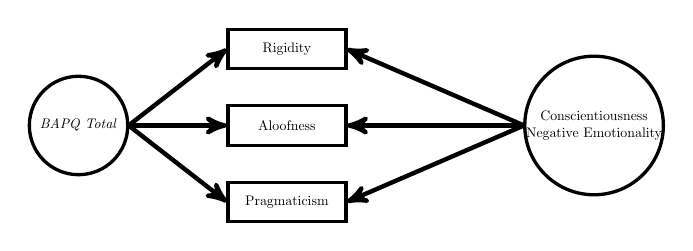
\begin{tikzpicture}[scale=.5,transform shape,auto,node distance=.9cm,
latent/.style={circle,draw,very thick,inner sep=0pt,minimum size=25mm,align=center},
manifest/.style={rectangle,draw,very thick,inner sep=0pt,minimum width=30mm,minimum height=10mm},
paths/.style={->, ultra thick, >=stealth'}]
\node [manifest] (SI) at (0,0) {Rigidity};
\node [manifest] (VO) [below=of SI] {Aloofness};
\node [manifest] (CO) [below=of VO] {Pragmaticism};
\node [latent] (g) [left=2.5cm of VO] {\emph{BAPQ Total}};
\node [latent] (Gc) [right=4.5cm of VO] {Conscientiousness\\ Negative Emotionality};
\foreach \all in {SI, VO, CO}
{
\draw [paths] (g.east) to node { } (\all.west);
}
\foreach \vc in {SI, VO, CO}
\draw [paths] (Gc.west) to node {} (\vc.east);
\end{tikzpicture}
\caption{\label{fig:TikZmodel} Significant Correlational Relationships between Personality and ASD Traits.}
\end{figure}

It was determined that there was a clear focal distribution of resonant power in the frontal cortex (Figure~\ref{fig:FocalDist}).

\begin{figure}[h!] 
\centering
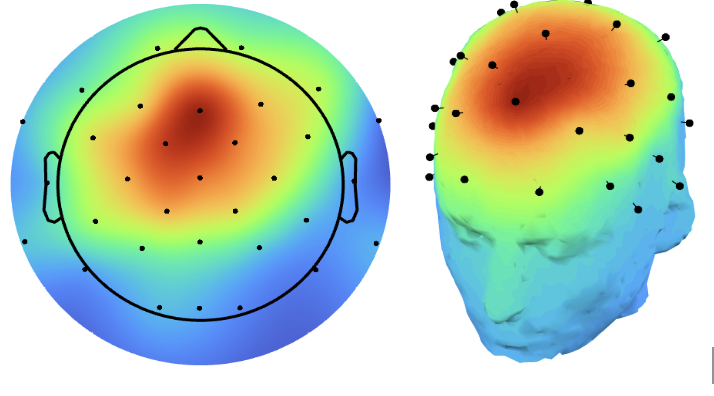
\includegraphics[width=0.3\textwidth]{Focal Dist.png}
\caption{\label{fig:FocalDist}EEG topographical maps of resonance peaks across all frequencies.}
\end{figure}

Descriptive statistics were computed for all key self-report measures, including the BAPQ subscales and the BFI-2S personality dimensions (see Table~\ref{tab:table1}).

\begin{table}[H]
\caption{Descriptive Statistics.}
\label{tab:table1}
 \begin{tabular}{l l c c c}
 \toprule
                          &              & \multicolumn{3}{c}{Week}\\
  \cmidrule{3-5}
                          &              & \textbf{One}    & \textbf{Two}    & \textbf{Three}\\
  \multirow{ 2}{*}{Group} & Experimental &     1008.435    &      986.76     &      859.1     \\
                          & Control      &     996.23      &      901.67     &      1002.23   \\
  \bottomrule
 \end{tabular}
\end{table}


\section{Discussion}
The present study aimed to evaluate whether binaural beats could be used to induce neural resonance at specific frequencies and whether individual differences in ASD, as measured by the BAPQ, are associated with individual variations in neural resonance profiles. Overall, the results supported the hypotheses that binaural beats would induce a significant increase in oscillatory power above that observed while listening to a pure tone at specific frequencies and that there were significant relationships between peak resonance frequencies and ASD traits. These findings suggest that binaural beats can induce frequency-coupled neural resonance across participants at a wide range of frequencies. Furthermore, the findings suggest that neural resonance profiles are significantly associated with social and affective processes related to ASD.




\bibliography{references.bib}

\end{document}
https://www.overleaf.com/project/64ef8e5b3faa92d4248ddcf9